\section{植物分类系统}

\subsection{植物的分类}

植物分类如\autoref{tab:clsfctn_vegetbls}所示。

\begin{table}[htbp]
	\centering
	\begin{NiceTabularX}{\textwidth}{cCCC}[hvlines]
		裸藻门 & \Block[v-center]{9-1}{藻类植物} & \Block[v-center]{13-1}{孢子植物} & \Block[v-center]{11-1}{低等植物} \\
		绿藻门 &  &  &  \\
		黄藻门 &  &  &  \\
		硅藻门 &  &  &  \\
		金藻门 &  &  &  \\
		甲藻门 &  &  &  \\
		褐藻门 &  &  &  \\
		红藻门 &  &  &  \\
		蓝藻门 &  &  &  \\
		黏菌门 & \Block[v-center]{2-1}{菌类} &  &  \\
		地衣门 &  &  &  \\
		苔藓植物门 & \Block[v-center]{2-1}{颈卵器植物} &  & \Block[v-center]{4-1}{高等植物} \\
		蕨类植物门 &  &  &  \\
		裸子植物门 & \Block[v-center]{2-1}{维管植物} & \Block[v-center]{2-1}{种子植物} &  \\
		被子植物门 &  &  & 
	\end{NiceTabularX}
	\caption{植物的分类}
	\label{tab:clsfctn_vegetbls}
\end{table}

\subsection{植物分类的阶层、双名法}

植物分类的各阶层见\autoref{tab:plant_class}。

\begin{table}[htbp]
	\centering
	\begin{tabularx}{\textwidth}{|C|C|C|c|}
		\hline
		中文 & 英文 & 拉丁文 & 词尾 \\ \hline
		植物界 & Vegetable Kingdom & Regnum Vegetabile &  \\ \hline
		门 & Division & Divisio, Phylum & -phyta \\ \hline
		亚门 & Subdivision & Subdivisio & -phytina \\ \hline
		纲 & Class & Classis & -eae, -opsida \\ \hline
		亚纲 & Subclass & Subclassis & -idae \\ \hline
		目 & Order & Ordo & -ales \\ \hline
		亚目 & Suborder & Subordo & -ineae \\ \hline
		科 & Family & Familia & -aceae \\ \hline
		亚科 & Subfamily & Subfamilia & -oideae \\ \hline
		族 & Tribe & Tribus & -eae \\ \hline
		亚族 & Subtribe & Subtribus & -inae \\ \hline
		属 & Genus & Genus & -a, -um, -us \\ \hline
		亚属 & Subgenus & Subgenus &  \\ \hline
		组 & Section & Sectio &  \\ \hline
		亚组 & Subsection & Subsectio &  \\ \hline
		系 & Series & Series &  \\ \hline
		亚系 & Subseries & Subseries &  \\ \hline
		种 & Species & Species &  \\ \hline
		亚种 & Subspecies & Subspecies &  \\ \hline
		变种 & Variety & Varietas &  \\ \hline
		亚变种 & Subvariety & Subvarietas &  \\ \hline
		变型 & Form & Forma &  \\ \hline
		亚变型 & Subform & Subforma &  \\ \hline
	\end{tabularx}
	\caption{植物各阶分类单元}
	\label{tab:plant_class}
\end{table}

植物命名采用双名法。学名=属名+种加词(+命名人)。属名和种加词都要用拉丁语或拉丁化的词来写。

命名人的书写有下列要点:
\begin{itemize}
	\item 命名人通常以其姓氏的缩写来表示,还要拉丁化。林奈(Linnaeus)的缩写为L.,单字母缩写仅限林奈一人。
	\item 当子女和父母均为命名人时,子女的姓氏缩写后加“f.”或“fil.”表示子女。
	\item 二人共同命名植物时,两人姓氏缩写中间加“et.”,意为“和”;多人命名,则在第一个人的姓氏缩写后加“et al.”或“etc.”。
	\item 如一学名由甲学者提出,但未经正式发表,又由乙学者正式发表,则把甲的姓氏放前面,用“ex”(从)连接乙的姓氏。
\end{itemize}

对于亚种或变种,应用三名法或四名法,即比双名法多了亚种和变种加词。

\begin{table}[htbp]
	\centering
	\begin{tabularx}{\textwidth}{|C|C||C|C|}
		\hline
		\textbf{缩写字} & \textbf{中文} & \textbf{缩写字} & \textbf{中文} \\ \hline
		comb. nov. & 新组合 & nov. sp. & 新种 \\ \hline
		cult. & 栽培的 & sect. & 组、节 \\ \hline
		cv. & 栽培变种,品种 & sp. nov. & 新种 \\ \hline
		et & 和、同、以及 & spp. & 许多种 \\ \hline
		ex & 从、出自 & subsp. 或 ssp. & 亚种 \\ \hline
		f. & 变型 & subgen. & 亚属 \\ \hline
		nom. nud. & 裸名 & syn. & 异名 \\ \hline
		var. & 变种 &  &  \\ \hline
	\end{tabularx}
	\caption{常见拉丁文缩写}
	\label{tab:latin_abbrs}
\end{table}

\subsection{国际植物命名法规}

国际植物命名法规(巴黎法规)的要点如下:
\begin{description}
	\item[模式标本] 种和种以下的分类群的命名必须有模式标本做根据。模式标本必须永久保存,所以不能是活植物。
	\item[唯一合法学名] 每一种植物只有一个合法的学名,其他名称应作为异名或废弃。
	\item[学名的格式] 学名包括属名和种加词,最后附加命名人之名。
	\item[学名的发表] 学名只有通过符合规定的方式发表才有效。
	\item[优先律原则] 凡是符合命名法规的最早发表的名称,就是唯一正确的名称。
	\item[学名的改变] 认为某属的一种植物应该转移到另一属中,可保留原来的种加词,这样形成的名称叫“新组合”,原有的名字叫基原异名。原命名人的名字用括号括起来,其后加上新学名的命名人。
	\item[保留名] 对于不符合命名法规的名称,有些沿用已久,经讨论作为保留名。
	\item[名称的废弃] 不符合规范的学名应该废弃。这包括将已废弃的属名作为种加词。
\end{description}

\section{藻类}

\subsection{蓝藻门}

\subsubsection{形态}

\begin{description}
	\item[胶质鞘] 细胞壁外面有果胶酸和粘多糖构成的胶质鞘,常含有非光合色素。
	\item[细胞壁] 分四层,最内层主要是肽聚糖,可被溶菌酶溶解,染色$\text{G}^{-}$。
	\item[集群状况] 有单细胞、群体和丝状体的。一些蓝藻藻丝上有异形胞,用于固氮,较大,细胞壁增厚以隔绝氧气。
	\item[细胞质] 分化为中心质(中央体)和周质(色素质)两部分。DNA聚集在中心质。
\end{description}

\subsubsection{光合}

\begin{description}
	\item[场所] 无载色体,只有光合片层。
	\item[光合色素] 叶绿素a、藻蓝蛋白、藻红蛋白、黄色色素。
	\item[光合产物] 蓝藻淀粉、藻青素颗粒体。
\end{description}

\subsubsection{繁殖}

\begin{description}
	\item[营养繁殖] 
	
	\begin{itemize}
		\item 单细胞:单细胞类型的蓝藻,发生分裂后子细胞立即分离。
		\item 藻殖段:丝状体蓝藻,以死细胞、异形胞或外力作用将丝状体分为几个小段,分别发育为新个体;
		\begin{figure}[htbp]
			\centering
			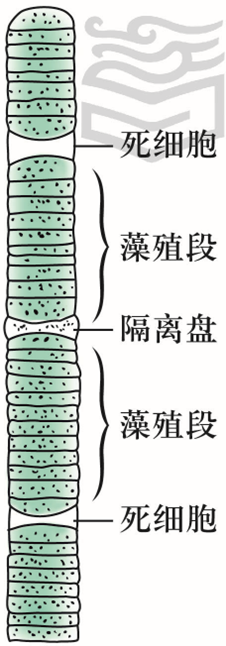
\includegraphics[width=0.2\textwidth]{Pics/藻殖段}
			\caption{藻殖段}
			\label{fig:zaozhiduan}
		\end{figure}
	\end{itemize}
	\item[无性生殖] 
	
	\begin{itemize}
		\item 厚壁孢子:除颤藻科之外的丝状类型产生,由普通营养细胞积累营养物质和细胞壁增厚而来;
		\item 外生孢子:管胞藻目产生,细胞横分裂为不等的两部分,小的形成孢子,大的不断分裂成大小两部分;
		\item 内生孢子:管胞藻目产生,母细胞增大,多次分裂,最后破裂释放出孢子。
		\begin{figure}[htbp]
			\centering
			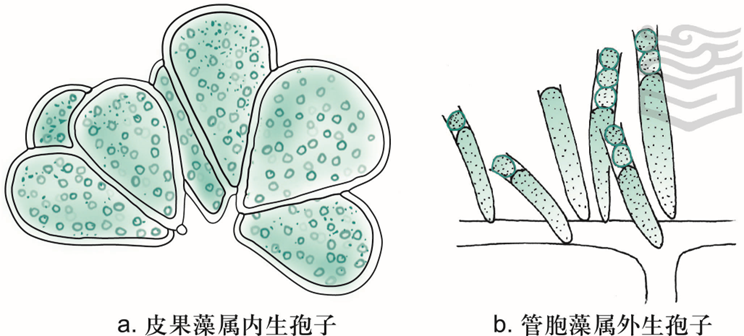
\includegraphics[width=0.7\linewidth]{Pics/内生孢子和外生孢子}
			\caption{内生孢子和外生孢子}
			\label{fig:exospore_endospore}
		\end{figure}
		
	\end{itemize}
\end{description}

\subsubsection{分类}

\paragraph{单细胞或群体类型的代表}

\subparagraph{色球藻属}

属于色球藻目单细胞或群体,外有胶质鞘。群体是多代子细胞在一起形成的。每个细胞有个体胶质鞘,还有共同的群体胶质鞘。(\autoref{fig:chroococcus})

\begin{figure}[htbp]
	\centering
	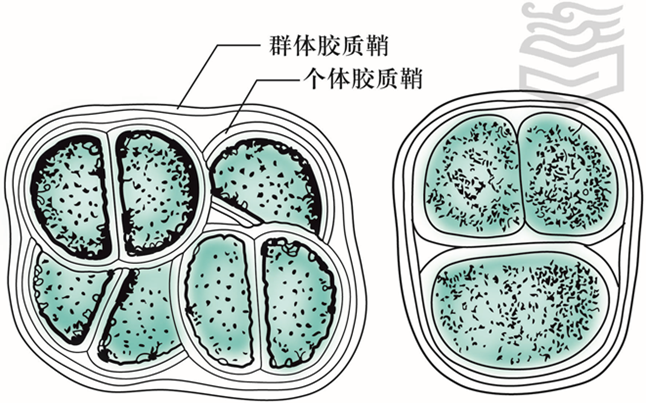
\includegraphics[width=0.5\linewidth]{Pics/色球藻属的胶质鞘}
	\caption{色球藻属的胶质鞘}
	\label{fig:chroococcus}
\end{figure}

\subparagraph{微囊藻属}

属于色球藻目。植物体球形、不规则或是有很多穿孔的浮游群体。(\autoref{fig:microcystis})群体细胞均匀分布在无结构的基质中。

微囊藻可以产生抑制其他藻类生长的物质。有的种类还可以产生“致死因子”这一毒素,毒害摄食藻类的动物。

夏季微囊藻大量繁殖形成\sy{水华}。

\begin{figure}[htbp]
	\centering
	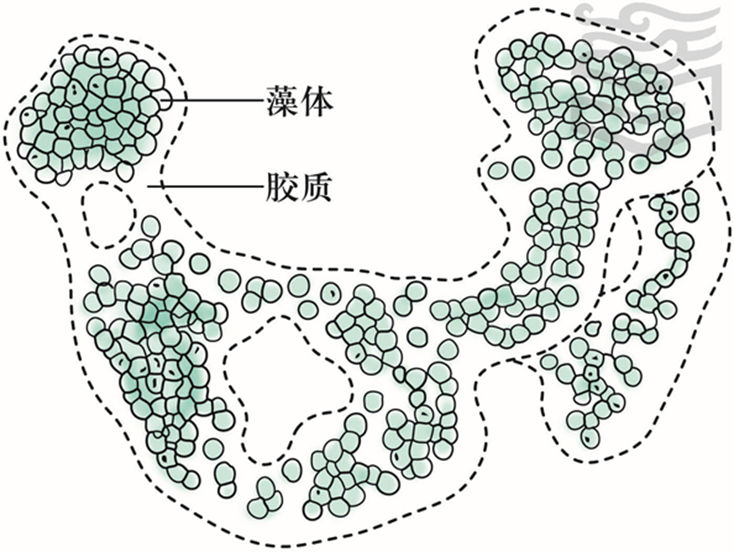
\includegraphics[width=0.6\linewidth]{Pics/微囊藻属}
	\caption{微囊藻属}
	\label{fig:microcystis}
\end{figure}

\subparagraph{管胞藻属}

属于管胞藻目。长杆型单细胞,有极性,以基部附生于其他水生植物上。产生外生孢子繁殖。

管胞藻目的皮果藻属以内生孢子繁殖。

\paragraph{丝状体的代表}

\subparagraph{颤藻属}

属于颤藻目。无胶质鞘或不明显。以藻殖段繁殖。注意席藻属容易与颤藻属混淆,区别是席藻属有胶质鞘。

\begin{figure}[htbp]
	\centering
	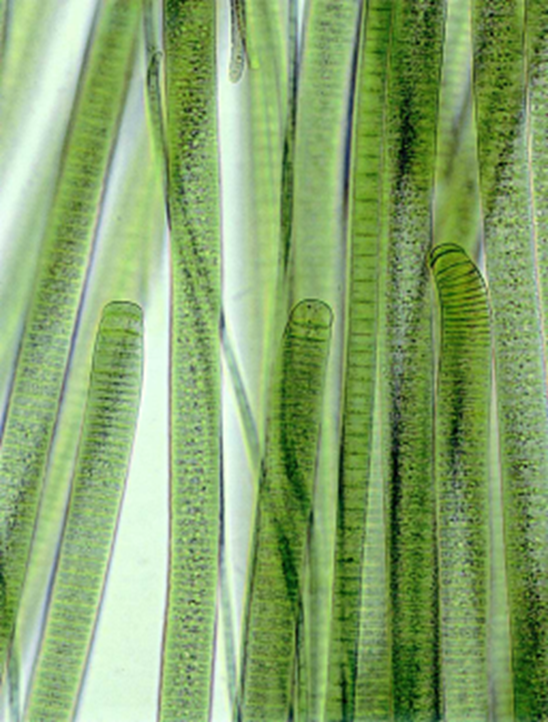
\includegraphics[width=0.4\linewidth]{Pics/颤藻属}
	\caption{颤藻属}
	\label{fig:oscillatoria}
\end{figure}


\subparagraph{念珠藻属}

属于颤藻目。丝状体常常无规则地集合在公共胶质鞘中。有时产生厚壁孢子。

地木耳和发菜都是本属的。

\begin{figure}[htbp]
	\centering
	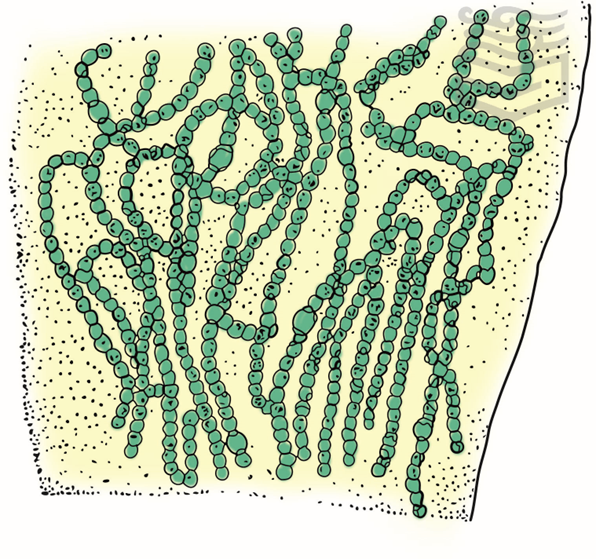
\includegraphics[width=0.3\linewidth]{Pics/念珠藻属}
	\caption{念珠藻属}
	\label{fig:nostoc}
\end{figure}


\subparagraph{鱼腥藻属}

属于颤藻目。和念珠藻属非常相似,区别是无公共胶质鞘。鱼腥藻常常与铜色微囊藻一同形成\sy{水华}。念珠藻和鱼腥藻都能固氮。

有一种鱼腥藻与红萍共生。

\begin{figure}[htbp]
	\centering
	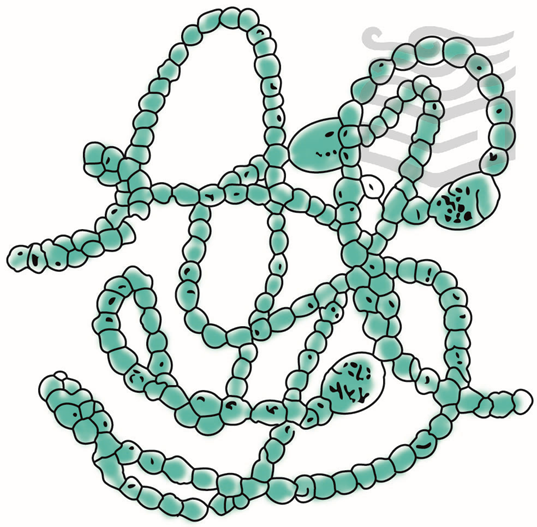
\includegraphics[width=0.3\linewidth]{Pics/鱼腥藻属}
	\caption{鱼腥藻属}
	\label{fig:anabeana}
\end{figure}


\subparagraph{真枝藻属}

属于颤藻目。许多丝状体聚集在一起,呈黑褐色绒毛状。胶质鞘坚硬、厚、透明,多为黄褐色。

\mbox{}

颤藻目中有些属具有假分支。如单歧藻属、双歧藻属。

\begin{figure}[htbp]
	\centering
	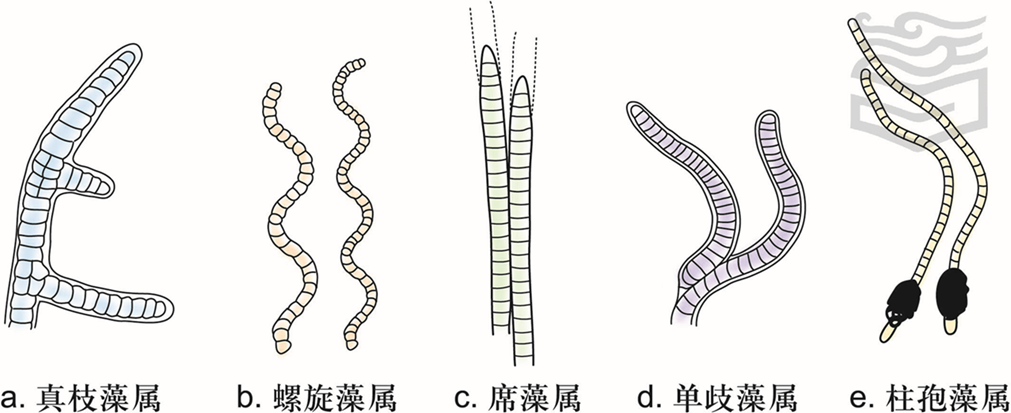
\includegraphics[width=0.7\linewidth]{Pics/真枝藻属等}
	\caption{真枝藻属等蓝藻}
	\label{fig:stigonema}
\end{figure}

\subsection{裸藻门}

\subsubsection{形态}

除了胶柄藻属,裸藻都是无细胞壁、有鞭毛、自由生活的藻类。
\begin{description}
	\item[细胞壁] 除胶柄藻属之外,都无细胞壁;
	\item[周质体] 质膜内侧的蛋白质结构;
	\item[鞭毛] 鞭毛为茸鞭型,9(2)+2型微管,外有原生质膜形成的鞭毛鞘。胶柄藻属无鞭毛;
	\item[眼点] 在储蓄泡和胞咽之间的背面,由橙色油滴组成。含有$\beta$-胡萝卜素或其衍生物。眼点有趋光性。
	\item[细胞核] 核较原始。在分裂间期染色质就有凝缩。有丝分裂时核膜不解体。无染色体纺锤体。
	\item[其他结构] 囊壳、胞口、胞咽、伸缩泡、储蓄泡。
\end{description}

\subsubsection{光合}

\begin{description}
	\item[载色体] 有3层膜,最外面是内质网膜,里面两层是载色体膜。类囊体三条一束。有时有蛋白核。
	\item[光合色素] 叶绿素a、叶绿素b、$\beta$-胡萝卜素、3种叶黄素。
	\item[光合产物] 裸藻淀粉。只出现在细胞质中。
\end{description}

裸藻的无色类型营腐生或吞噬营养。

\subsubsection{繁殖}

\begin{description}
	\item[细胞纵裂] 细胞分裂先是着生鞭毛一段开始凹陷,细胞核开始有丝分裂,随后是鞭毛器和眼点分裂。载色体和裸藻淀粉均分。一个子细胞保留鞭毛,另一个自己长出鞭毛。
	\item[胞囊] 分泌厚壁,形成胞囊渡过恶劣环境。
\end{description}

\subsubsection{分布}

裸藻大多分布在淡水,少数在半咸水,很少在海水中。是水质污染的指示植物。可形成水华。有两个属的裸藻生活在两栖类消化管中。

\subsubsection{分类}

\paragraph{裸藻属}

属裸藻目。

\paragraph{胶柄藻属}

属于胶柄藻属。

\subsection{甲藻门}

\subsubsection{形态}

\begin{description}
	\item[集群] 大多数甲藻是单细胞;少数为丝状体。
	\item[细胞壁] 有的没有细胞壁。细胞壁含纤维素,在纵裂甲藻为两个半片、横裂甲藻为多个板片。
	\item[细胞核] 核很大。即使在分裂间期染色质也浓缩。组蛋白很少。DNA间断复制。 
\end{description}

\section{菌类}

\begin{figure}
	\centering
	\begin{forest}
		forest scheme
		[菌类
			[黏菌门
				[黏菌纲]
				[集孢黏菌纲]
				[根肿菌纲]]
			[真菌门
				[鞭毛菌亚门]
				[接合菌亚门]
				[子囊菌亚门]
				[担子菌亚门]
				[半知菌亚门]]]
	\end{forest}
	\caption{菌类的分类}
	\label{fig:菌类的分类}
\end{figure}

\subsection{黏菌门}

\subsubsection{黏菌门的主要特征}

黏菌在生长期是变形体,即裸露无细胞壁、多核原生质团,与变形虫相似。繁殖时期产生具细胞壁的孢子。

黏菌是介于动物和植物之间的生物。

\subsubsection{黏菌门的主要类群}

\paragraph{黏菌纲}

黏菌纲有真正的变形体,产生具鞭毛的游动细胞,子实体外有包被。

黏菌纲常见的为发网菌属(\autoref{fig:发网菌})。营养体称变形体。

\begin{figure}[htbp]
	\centering
	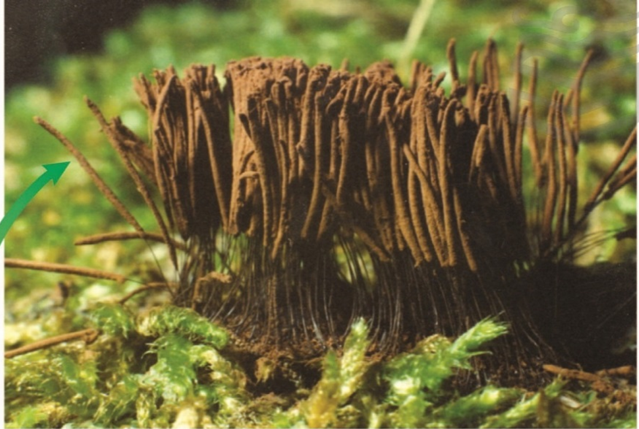
\includegraphics[width=0.5\linewidth]{Pics/发网菌}
	\caption{发网菌}
	\label{fig:发网菌}
\end{figure}


繁殖时,发网菌爬到光亮地方,形成发状突起,最后发育为孢子囊(子实体),外有包被。

孢子萌发为具2条不等长鞭毛的游动细胞。鞭毛收起来,就形成变形菌胞。形成合子后不休眠,多次有丝分裂后形成多核变形体。(\autoref{fig:发网菌的生活史})

\begin{figure}[htbp]
	\centering
	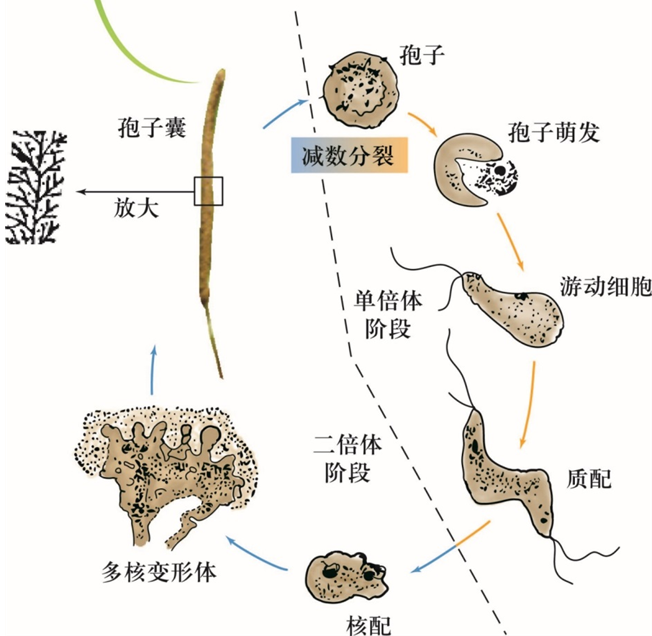
\includegraphics[width=0.6\linewidth]{Pics/发网菌的生活史}
	\caption{发网菌的生活史}
	\label{fig:发网菌的生活史}
\end{figure}

\paragraph{根肿菌纲}

寄生于高等植物、藻类或真菌。

不形成子实体。

芸薹根肿菌寄生于十字花科植物。

\subsection{真菌门}

\subsubsection{真菌的共同特征}

\paragraph{异养}

\begin{description}
	\item[寄生] 从活的动物、植物吸取养分;
	\item[腐生] 从动植物尸体、无生命的有机物质吸取养分;
	\item[兼性腐生] 寄生为主,兼腐生;
	\item[兼性寄生] 腐生为主,兼寄生。
	\item[专性腐生] 只可腐生;
	\item[专性寄生] 只能寄生;
\end{description}

很多真菌都是先寄生在活体上,活体死亡后就由寄生转为腐生。

\paragraph{营养体}

除单细胞真菌之外,都是由菌丝构成的。菌丝分为无隔菌丝和有隔菌丝两种。(\autoref{fig:有隔菌丝和无隔菌丝})

\begin{figure}
	\centering
	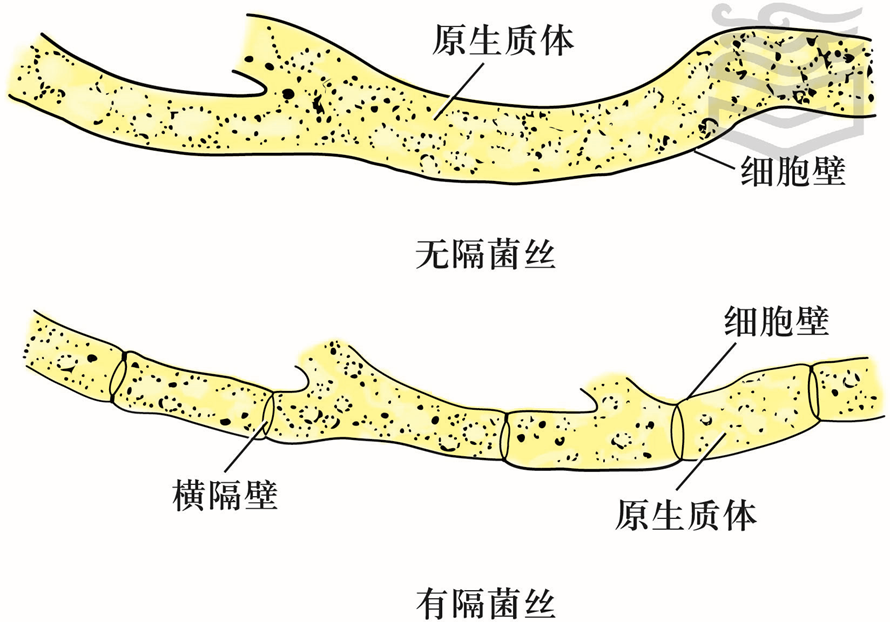
\includegraphics[width=0.7\linewidth]{Pics/菌丝的种类}
	\caption{有隔菌丝和无隔菌丝}
	\label{fig:有隔菌丝和无隔菌丝}
\end{figure}

绝大部分真菌都有细胞壁。

菌丝还是吸取养分的机构。

某些真菌在不良环境或繁殖的时候,菌丝相互密结,形成\sy{菌丝组织体}。包括根状菌索、菌核、子座几种类型。其中根状菌索和菌核是抵抗不良环境的,子座是营养阶段到繁殖阶段的过渡形式。(\autoref{fig:菌丝组织体})

\begin{figure}[htbp]
	\centering
	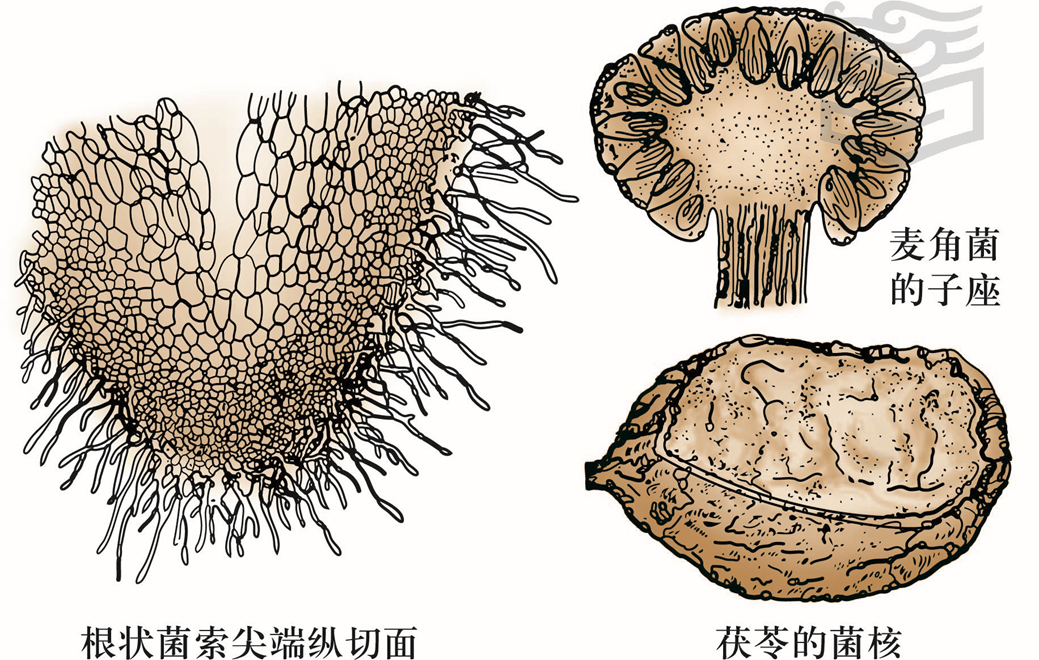
\includegraphics[width=0.6\linewidth]{Pics/菌丝组织体}
	\caption{菌丝组织体}
	\label{fig:菌丝组织体}
\end{figure}

\paragraph{繁殖}

\subparagraph{营养繁殖}

营养繁殖可产生下列孢子:(\autoref{fig:真菌营养繁殖和无性生殖的各种孢子})

\begin{description}
	\item[芽生孢子] 从单个细胞出芽产生,脱离母体后长成新个体。
	\item[厚壁孢子] 菌丝中个别细胞膨大形成休眠孢子,渡过不良环境后再萌发。
	\item[节孢子] 菌丝细胞断裂形成。
\end{description}

\subparagraph{无性生殖}

真菌通常进行无性生殖,可产生下列孢子:(\autoref{fig:真菌营养繁殖和无性生殖的各种孢子})
\begin{description}
	\item[游动孢子] 水生真菌的孢子;
	\item[孢囊孢子] 在孢子囊内形成的不动孢子,借风传播;
	\item[分生孢子] 分生孢子囊梗产生的不动孢子,借动物或风传播。
\end{description}

\begin{figure}[htbp]
	\centering
	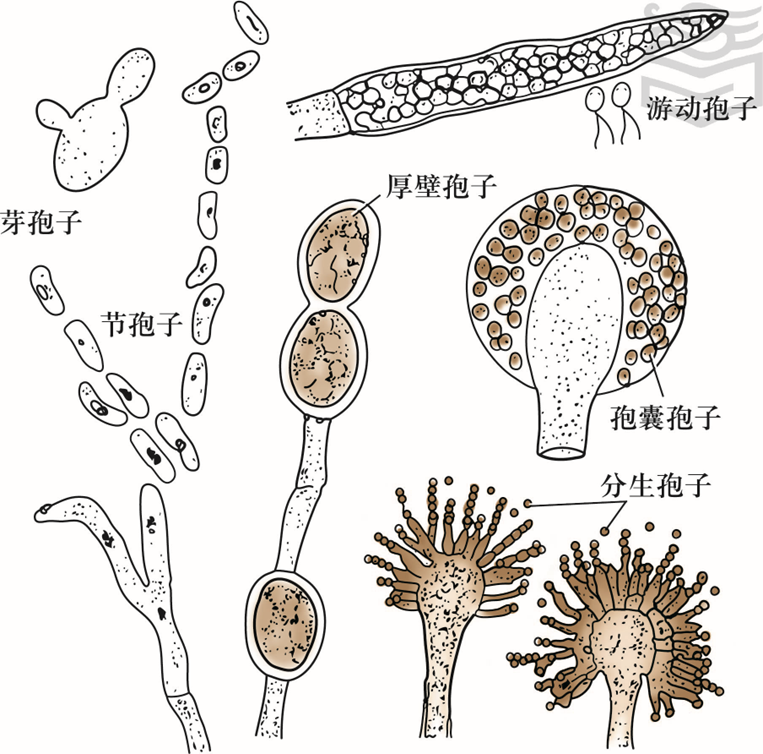
\includegraphics[width=0.\linewidth]{Pics/真菌营养繁殖和无性生殖的各种孢子}
	\caption{真菌营养繁殖和无性生殖的各种孢子}
	\label{fig:真菌营养繁殖和无性生殖的各种孢子}
\end{figure}


\subparagraph{有性生殖}

低等的真菌为配子的配合,有同配、异配之别。

有些真菌形成精囊和卵囊,精卵结合形成卵孢子。

子囊菌有性配合形成子囊,内有子囊孢子。担子菌有性配合后,在担子上形成担孢子。子囊孢子和担孢子都是有性孢子,和无性生殖的孢子完全不同。

\paragraph{生活史}

在真菌的生活史中,二倍体只是一个合子,并不是一个营养体,所以真菌只有核相交替,无世代交替。

\subsubsection{真菌门的主要类群}

\paragraph{鞭毛菌亚门}

主要特征:  

\begin{description}
	\item[形态] 大部分是分枝的丝状体,菌丝无隔。少部分为单细胞。
	\item[无性生殖] 产生\zhongdian{具鞭毛}的游动孢子。
	\item[有性生殖] 产生卵孢子或休眠孢子。低等种类是同配或异配生殖。
\end{description}


\section{地衣}

地衣是真菌和藻类的共生体,真菌多为子囊菌,少数为担子菌,极少数为半知菌。藻类为绿藻或蓝藻。

地衣的形态几乎完全是真菌控制的。藻类给真菌提供光合产物,真菌给藻类提供水分和无机盐,